%----------------------------------------------------------------------
% Introduction
%----------------------------------------------------------------------

\section{Introduction}

\begin{frame}{Why do we have programming assignments?}
\begin{itemize}
\item Distribute marks outside of exams
\item Apply topics learned in class
\end{itemize}
\end{frame}

\note{
\begin{itemize}
\item To start, we ask why do we even need assignments in programming courses? If not, then this entire project is moot
\item Broadly speaking there are two reasons:
\begin{itemize}
\item From a practical POV, it's easy way to assign marks
\item From a holistic POV, we want students to apply the knowledge they learned in class
\end{itemize}
\end{itemize}
}

%----------------------------------------------------------------------

\begin{frame}{How do we mark assignments?}
\begin{block}{Automated I/O Testing (Lower-year courses)}
Simple algorithms
\end{block}
\begin{block}{Manual Checking (Upper-year courses)}
Advanced algorithms
\end{block}
\end{frame}

\note{
\begin{itemize}
\item Now that we know why we need assignments, the question then becomes how do we mark them?
\item There are two general approaches to marking:
\begin{itemize}
\item First is automated IO testing
\item Mostly done in lower year courses where the assignments involve simple algorithms like implement sorting
\item We can then check for correctness by providing test cases and diffing the output with expected output
\item This type of testing is not as common in upper year courses where the algorithms are more advanced like concurrency, operating systems, networking, computer graphics, etc. A few exceptions still exist like advanced algorithms and compiler construction
\end{itemize}
\end{itemize}
}

%----------------------------------------------------------------------
% Problem
%----------------------------------------------------------------------

\subsection{Problem}

\begin{frame}{Problem}
\begin{block}{Why can't we just hire more TAs?}
Not scalable for thousands of students
\end{block}
\begin{itemize}
\item Inconsistent
\item Tedious
\item Error-prone
\end{itemize}
\end{frame}

\note{
\begin{itemize}
\item So you might be wondering what's the problem with manual marking? As class sizes grow, we will get more tuition money, which can then be used to hire more TAs
\item Speaking from experience, I'd say hiring more TAs is not scalable beyond more than a hundred students or so
\begin{itemize}
\item The more TAs you hire, the more inconsistent marking becomes. One might be generious and another might not be so you'd end up with students complaining that their friend received more marks for the same answer
\item If we were to assign one TA per assignment for consistency, then it becomes incredibly tedious and time consuming to mark hundreds/thousands of the same assignment
\item Finally, manual marking becomes more problematic depending on the topic. Student networking/operating systems code can be extremely difficult to comprehend
\end{itemize}
\end{itemize}
}

%----------------------------------------------------------------------
% Motivating Example
%----------------------------------------------------------------------

\subsection{Motivating Example}

\begin{frame}{Motivating Example}{ECE459 A1: Paster Assignment}
\begin{center}
\begin{tikzpicture}
\tikzset{Node/.style={shape=rectangle, draw, align=center}}
\tikzset{Edge/.style={-latex, bend right=-90, above, sloped}}
\node [Node] (client) {C Client};
\node []     ()       [left=1cm, label={Image 1}]{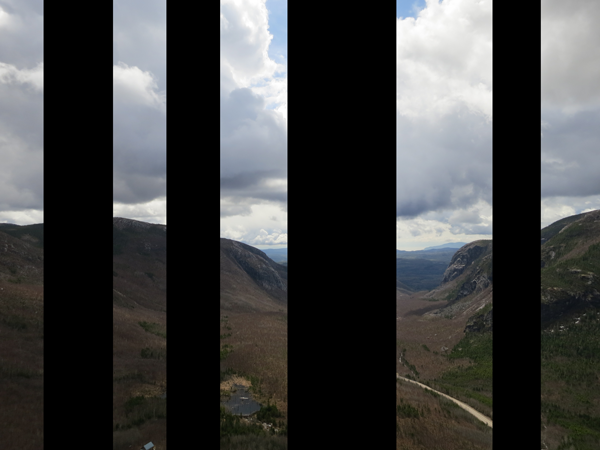
\includegraphics[height=2cm]{presentation/total}};
\node [Node] (server) [right=5cm]{Web Server};
\path [Edge] (client.north) edge node[above]{\texttt{GET :4590/image?img=1}} (server.north);
\path [Edge] (server.south) edge node[below, yshift=1cm, label={Random Fragment $i$}]{
\includegraphics[height=2cm]{presentation/slice}} (client.south);
\end{tikzpicture}
\end{center}
\end{frame}

\note{
\begin{itemize}
\item The motivating example I've used for my project is the first assignment in ECE459
\item In this assignment, students are provided with a serial version of the client program and their task is to rewrite it once with non-blocking IO and again with pthreads.
\item This program is essentially just a loop that calls our webserver that, after a random delay, returns a random fragment of an image. The response header will contain the index of the fragment. The client will loop until all the fragments have been received and so that it can reconstruct the image.
\end{itemize}
}

%----------------------------------------------------------------------

\begin{frame}{Why can't we use automated marking?}
\begin{block}{Input/Output Testing?}
\begin{itemize}
\item Sample program and expected program have the same input/output
\end{itemize}
\end{block}
\begin{block}{Checking CPU Usage?}
\begin{itemize}
\item Easy to fake busy-waiting threads
\end{itemize}
\end{block}
\begin{block}{Checking CPU Runtimes?}
\begin{itemize}
\item Non-deterministic network calls
\end{itemize}
\end{block}

\end{frame}

\note{
\begin{itemize}
\item So you might be wondering why we can't use automated testing for this assignment
\item We can't do IO testing other than baseline checking for correctness because both the provided sample program and expected program have the same input/outputs
\item We can't check CPU usage because it's easy to fake busy-waiting threads
\item We also can't check runtimes because the total runtime is non-deterministic due to the network calls
\item And finally, we occasionally get students that complain about penalizing poor runtimes due to bad programming habits -- ironic for a course called programming for performance
\end{itemize}
}

%----------------------------------------------------------------------
% ClangAutoMarker
%----------------------------------------------------------------------

\subsection{ClangAutoMarker}

\begin{frame}{ClangAutoMarker}
\begin{itemize}
\item Correct solutions should have similar ASTs
\item Compare student solutions to reference solutions to automatically grade them
\end{itemize}
\end{frame}

\note{
\begin{itemize}
\item Now I can finally discuss the ClangAutoMarker tool that I have built for my masters thesis
\item I hypothesized that correct solutions will have more similar ASTs to reference solutions than incorrect solutions
\item The idea is to programatically compare student solutions with reference solutions to automatically grade them
\end{itemize}
}
